\begin{task}{441}
Перечислите все попарно неизоморфные связные простые графы на \(8\) вершинах, в которых ровно три блока и при этом не более двух простых циклов. Подробно описывать перебор не нужно (не нужно описывать получение каждого отдельного графа), но обязательно стоит разделить графы на группы по значениям параметров, по которым осуществлялся перебор (параметров должно быть минимум два, второй из которых позволяет перебирать графы с одинаковым значением первого параметра). При переборе случаев используйте вложенные окружения \textbf{enumerate} и окружение \textbf{figure}, не забудьте также использовать пары команд \textbf{ref} и \textbf{label} для описания рисунков. Описание случаев перебора должно происходить в тексте решения в tex-файле, а не внутри рисунков!
\end{task}

\begin{solution}

Будем пользоваться следующими определением и теоремой:

\begin{definition}\label{определение блок}
Блок~--- это максимальный подграф графа, не имеющий собственных точек сочленения (другими словами, некоторые точки сочленения графа могут принадлежать блоку, но своих точек сочленения у блока нет).
\end{definition}

\begin{theorem}\label{теорема цикл вершин блока}
В блоке с не менее чем тремя вершинами любые две из них связаны простым циклом.
\end{theorem}
\begin{proof}
Во-первых, заметим, что, если количество вершин в блоке меньше трех, цикла в нем быть не может.

Далее рассмотрим две вершины блока: $u$ и $v$. Обозначим $d(u,~v)$ как кратчайшее расстояние между ними.
\begin{enumerate}
    \item \label{$d(u,v)=1$} Если $d(u,~v) = 1$, значит, вершины смежны, причем ребро $(u,~v)$ не мост, иначе одна из вершин окажется точкой сочленения, что противоречит определению~\ref{определение блок}. Тогда существует простой цикл, проходящий через ребро $(u,~v)$, ведь при его удалении всё равно найдется цепь, соединяющая вершины $u$ и $v$.
    \item Пусть теперь $d(u,~v) > 1$. Возьмем кратчайший путь из $u$ в $v$, обозначив за $t$ предпоследнюю вершину этого пути. Тогда получим $d(u,~t) = d(u,~v) - 1$.
    
    Воспользуемся методом математической индукции и предположим, что уже существует простой цикл $C$, содержащий вершины $u$ и $t$.
    
    Так как $d(t,~v) = 1$, из п.~\ref{$d(u,v)=1$} получаем, что $t$ не точка сочленения, значит, есть простой путь $P$, соединяющий вершины $u$ и $v$ и не проходящий через $t$. Пусть $w$~--- первая вершина пути $P$ из $v$ в $u$, которая принадлежит $C$ (она точно существует, потому что $u \in C$). Получаем цикл, состоящий из:
    \begin{enumerate}
        \item части пути $P$ из $v$ в $w$;
        \item части цикла $C$ из $w$ в $t$, проходящей через $u$;
        \item ребра $(t,~v)$.
    \end{enumerate}
\end{enumerate}

\begin{figure}[H]
    \centering
    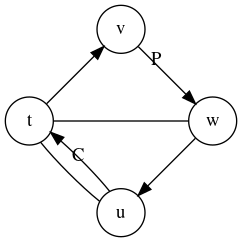
\includegraphics[scale=0.5]{Fall/img/solution-441_cycle_for_the_theorem.dot.png}
    \caption{Иллюстрация к доказательству теоремы (стрелками показан цикл).} \label{cycle for the theorem}
\end{figure}

База индукции уже установлена в п.~\ref{$d(u,v)=1$}, а также доказан переход: при предположении существования простого цикла, содержащего вершины $u$ и $t$, существует простой цикл, содержащий вершины $u$ и $v$, причем $d(u,~t) = d(u,~v) - 1$. Теорема доказана.
\end{proof}

Заметим, что граф на \(8\) вершинах должен содержать ровно три блока, значит, он имеет ровно две точки сочленения, условно разделяющих граф на блоки.

Теперь рассмотрим структуру блоков более подробно. Во-первых, необходимо

\begin{proposition}\label{k-цикл}
Если в блоке, содержащем $n$ вершин, есть простой цикл, содержащий меньшее количество вершин, то в блоке есть как минимум три различных простых цикла.
\end{proposition}
\begin{proof}
Занумеруем шаги наших рассуждений:
\begin{enumerate}
    \item Блок, содержащий три вершины, единственен: он должен быть полным, иначе одна из вершин окажется точкой сочленения, что противоречит определению~\ref{определение блок}.
    
    \item Допустим, при $n > 3$ нас есть $n$-блок, в котором есть цикл содержащий $k < n$ вершин (для удобства занумеруем их числами от \(1\) до \(k\)). Так как граф связный, остальные вершины с номерами от $k + 1$ до $n$ должны быть связаны с циклом, причем как минимум две из этих вершин точно должны иметь ребра, связывающие их с $k$-циклом, ведь в противном случае либо граф перестанет быть связным (ни одна из вершин с номерами, большими $k$ не связана с циклом ребром), либо найдется точка сочленения, что противоречит определению~\ref{определение блок} (одна вершина $x$ связана с вершиной цикла $y$ ребром, а остальные связаны с $x$ и/или между собой~--- тогда $y$ станет точкой сочленения).
    
    Получили, что как минимум две вершины связаны с $k$-циклом.
    
    \item Пусть у нас есть группа связанных между собой вершин $G$.
    
    \begin{enumerate}
        \item Если $|G| = 1$, другими словами, там только одна вершина $u$, значит, она должна быть связана как минимум двумя  ребрами с вершинами $k$-цикла (пусть это, условно, будут вершины $a$ и $b$). Тогда у нас есть минимум три цикла: ребра $(a,~u), (u,~b)$ и путь, соединяющий по циклу вершины $b$ и $a$; ребра $(a,~u), (u,~b)$ и путь, соединяющий по циклу вершины $a$ и $b$ (здесь уже берем другую часть цикла); исходный $k$-цикл.
        
        \begin{figure}[H]
            \centering
            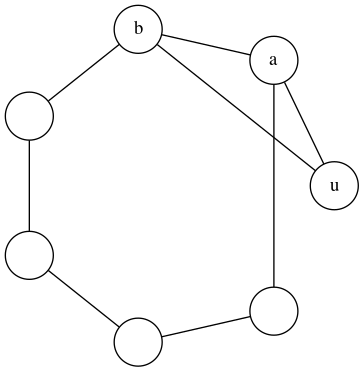
\includegraphics[scale=0.4]{Fall/img/solution-441_for_the_proposition.dot.png}
            \caption{Иллюстрация к доказательству утверждения $(a)$.} \label{cycle for the theorem b}
        \end{figure}
        
        \item Если же $|G| > 1$, то в ней найдется две вершины $u$ и $v$, соединенные с $k$-циклом ребрами, а также между собой. Рассуждения по нахождению трех циклов аналогичные, но уже с использованием пути, соединяющего $u$ и $v$ и не содержащего ребер $k$-цикла.
    \end{enumerate}
    
    С учетом существования $k$-цикла имеем минимум три уникальных цикла внутри блока. Значит при наличии в $n$-блоке $k$-цикла ($k < n$), в нём будут как минимум три цикла.
\end{enumerate}
\end{proof}

По утверждению~\ref{k-цикл} в $n$-блоке должен быть только $n$-цикл! А для любого $n > 2$ найти такие блоки~--- тривиальная задача. По сути мы получаем простое <<кольцо>> $n$ ребер, соединяющих $n$ вершин. Кстати говоря, это также означает, что каждый блок на $n > 3$ вершинах содержит ровно один цикл!

Так как по условию должно быть ровно три блока и не более двух циклов, а из теоремы~\ref{теорема цикл вершин блока} любой блок, содержащий не менее трех вершин, также содержит и цикл, получаем, что как минимум один из наших блоков должен состоять из двух вершин, другими словами, должен быть мостом (обе его вершины~--- точки сочленения). Также по утверждению~\ref{k-цикл} два других блока дадут нам необходимые два или менее цикла. Осталось перебрать тройки блоков: за параметр мы возьмем количество вершин в каждом из них. Исключая симметрию (например, тройки блоков $(2,~3,~5)$ и $(5,~3,~2)$ изоморфны), получаем семь вариантов, перечисленных на рисунках:
\begin{table}[H]
\centering
$
\begin{array}{|c|c|c|c|c|c|c|c|}
	\hline
	\text{Блок} & (2,~3,~5) & (2,~5,~3) & (2,~2,~6) & (2,~6,~2) & (3,~2,~5) & (2,~4,~4) & (4,~2,~4)\\
	\hline
	\text{Рисунок} & \ref{group 2-3-5} & \ref{group 2-5-3} & \ref{group 2-2-6} & \ref{group 2-6-2} & \ref{group 3-2-5} & \ref{group 2-4-4} & \ref{group 4-2-4}\\
	\hline
\end{array}
$
\caption{Ссылки на рисунки.} \label{groups refs}
\end{table}

Но и это еще не все! Две точки сочленения могут располагаться друг от друга на разном расстоянии в случае, когда средний блок имеет $n \geqslant 4$ вершин. Получаем как раз-таки два параметра поиска неизоморфных графов: количество вершин в тройке блоков, кратчайшее расстояние между точками сочленения. Изобразим итоговые варианты на рисунках (если $a, b, c$~--- количество вершин в трёх блоках, а $d$~--- кратчайшее расстояние между точками сочленения:

% (2, 3, 5) --- 1
\begin{figure}[H]
    \centering
    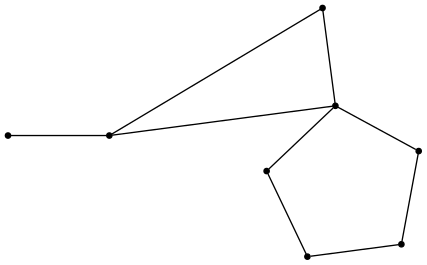
\includegraphics[scale=0.4]{Fall/img/solution-441_235_0.dot.png}
    \caption{Граф 2-3-5} \label{group 2-3-5}
\end{figure}

% (2, 5, 3) --- 3
\begin{figure}[H]
    \centering
    \begin{subfigure}[b]{0.45\linewidth}
        \centering
        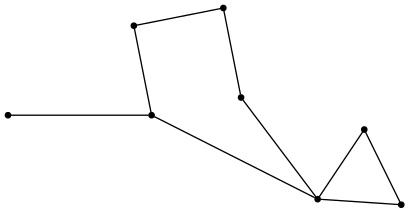
\includegraphics[scale=0.4]{Fall/img/solution-441_253_1.dot.png}
        \caption{Граф 2-5-3.1} \label{graph 2-5-3.1}
    \end{subfigure}
    \begin{subfigure}[b]{0.45\linewidth} 
        \centering
        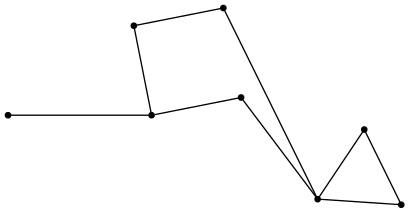
\includegraphics[scale=0.4]{Fall/img/solution-441_253_2.dot.png}
        \caption{Граф 2-5-3.2} \label{graph 2-5-3.2}
    \end{subfigure}
    \begin{subfigure}[b]{0.45\linewidth} 
        \centering
        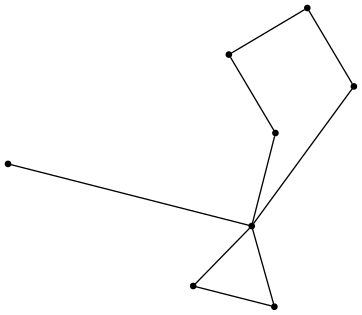
\includegraphics[scale=0.4]{Fall/img/solution-441_253_3.dot.png}
        \caption{Граф 2-5-3.3} \label{graph 2-5-3.3}
    \end{subfigure}
    
    \caption{Графы 2-5-3} \label{group 2-5-3}
\end{figure}

% (2, 2, 6) --- 1
\begin{figure}[H]
    \centering
    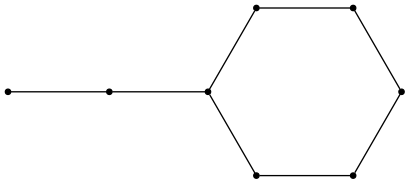
\includegraphics[scale=0.4]{Fall/img/solution-441_226_0.dot.png}
    \caption{Граф 2-2-6} \label{group 2-2-6}
\end{figure}

% (2, 6, 2) --- 4
\begin{figure}[H]
    \centering
    \begin{subfigure}[b]{0.45\linewidth}
        \centering
        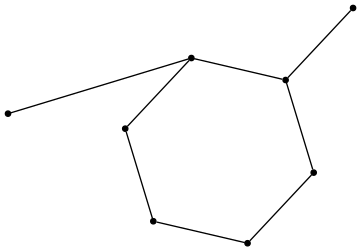
\includegraphics[scale=0.4]{Fall/img/solution-441_262_1.dot.png}
        \caption{Граф 2-6-2.1} \label{graph 2-6-2.1}
    \end{subfigure}
    \begin{subfigure}[b]{0.45\linewidth}
        \centering
        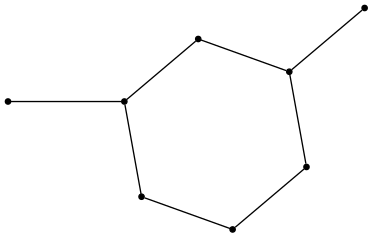
\includegraphics[scale=0.4]{Fall/img/solution-441_262_2.dot.png}
        \caption{Граф 2-6-2.2} \label{graph 2-6-2.2}
    \end{subfigure}
    \begin{subfigure}[b]{0.45\linewidth} 
        \centering
        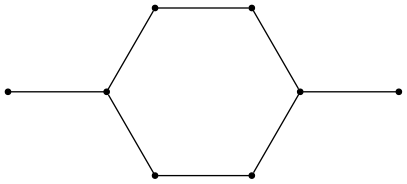
\includegraphics[scale=0.4]{Fall/img/solution-441_262_3.dot.png}
        \caption{Граф 2-6-2.3} \label{graph 2-6-2.3}
    \end{subfigure}
    \begin{subfigure}[b]{0.45\linewidth} 
        \centering
        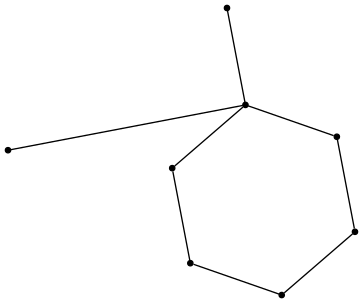
\includegraphics[scale=0.4]{Fall/img/solution-441_262_4.dot.png}
        \caption{Граф 2-6-2.4} \label{graph 2-6-2.4}
    \end{subfigure}
    
    \caption{Графы 2-6-2} \label{group 2-6-2}
\end{figure}

% (3, 2, 5) --- 1
\begin{figure}[H]
    \centering
    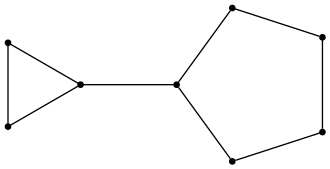
\includegraphics[scale=0.4]{Fall/img/solution-441_325_0.dot.png}
    \caption{Граф 3-2-5} \label{group 3-2-5}
\end{figure}

% (2, 4, 4) --- 3
\begin{figure}[H]
    \centering
    \begin{subfigure}[b]{0.45\linewidth}
        \centering
        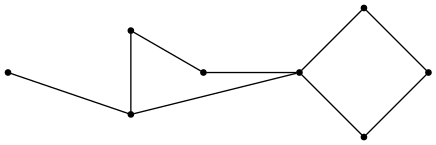
\includegraphics[scale=0.4]{Fall/img/solution-441_244_1.dot.png}
        \caption{Граф 2-4-4.1} \label{graph 2-4-4.1}
    \end{subfigure}
    \begin{subfigure}[b]{0.45\linewidth} 
        \centering
        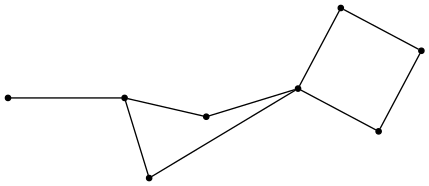
\includegraphics[scale=0.4]{Fall/img/solution-441_244_2.dot.png}
        \caption{Граф 2-4-4.2} \label{graph 2-4-4.2}
    \end{subfigure}
    \begin{subfigure}[b]{0.45\linewidth} 
        \centering
        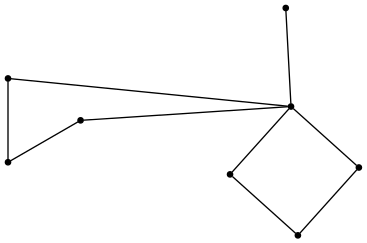
\includegraphics[scale=0.4]{Fall/img/solution-441_244_3.dot.png}
        \caption{Граф 2-4-4.3} \label{graph 2-4-4.3}
    \end{subfigure}
    
    \caption{Графы 2-4-4} \label{group 2-4-4}
\end{figure}

% (4, 2, 4) --- 1
\begin{figure}[H]
    \centering
    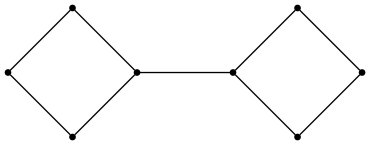
\includegraphics[scale=0.4]{Fall/img/solution-441_424_0.dot.png}
    \caption{Граф 4-2-4} \label{group 4-2-4}
\end{figure}

\textbf{Ответ:} Всего получаем 14 графов!

\end{solution}
